%!TEX root = ../colloquium.tex

\begin{frame}[plain,noframenumbering]
	\centering
	\vspace*{2.6cm}
	\Huge \colorit{Part II}
	\vskip 20pt
	\Large Steenrod barcodes
\end{frame}

\begin{frame}{Goal: introduce Steenrod barcodes}
	\pause
	These generalize usual barcodes, and are also
	\pause
	\colorit{stable},
	\pause
	\colorit{computable},
	\pause
	and present in \colorit{real-data}.

	\pause\medskip
	\vskip-15pt
	\begin{figure}
		\centering
		\begin{subfigure}[b]{0.49\textwidth}
			\centering
			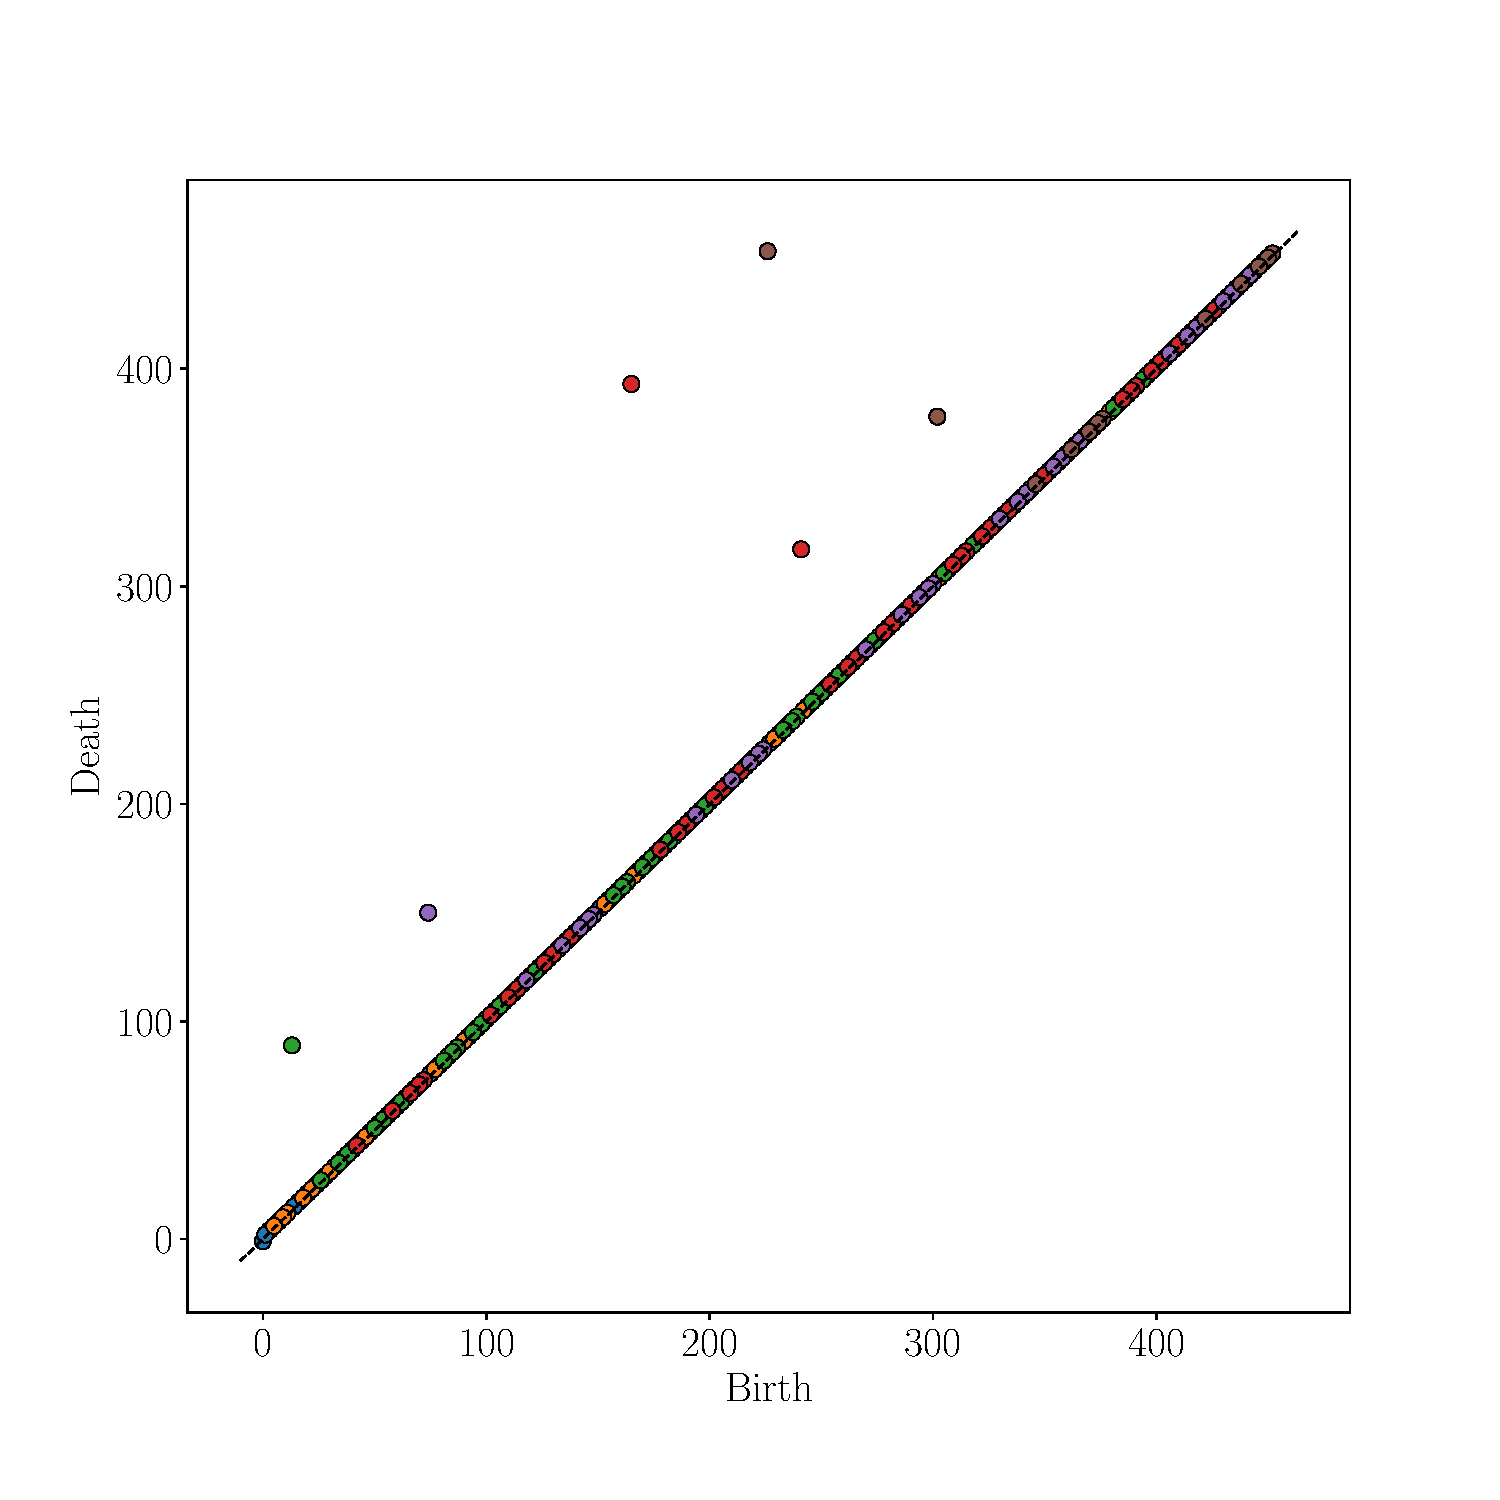
\includegraphics[width=\textwidth]{aux/s2_s4.pdf}
			\caption{$\mathrm C\,\Sigma(S^2 \vee S^4)$}
			\label{f:s2_s4}
		\end{subfigure}
		\pause
		\begin{subfigure}[b]{0.49\textwidth}
			\centering
			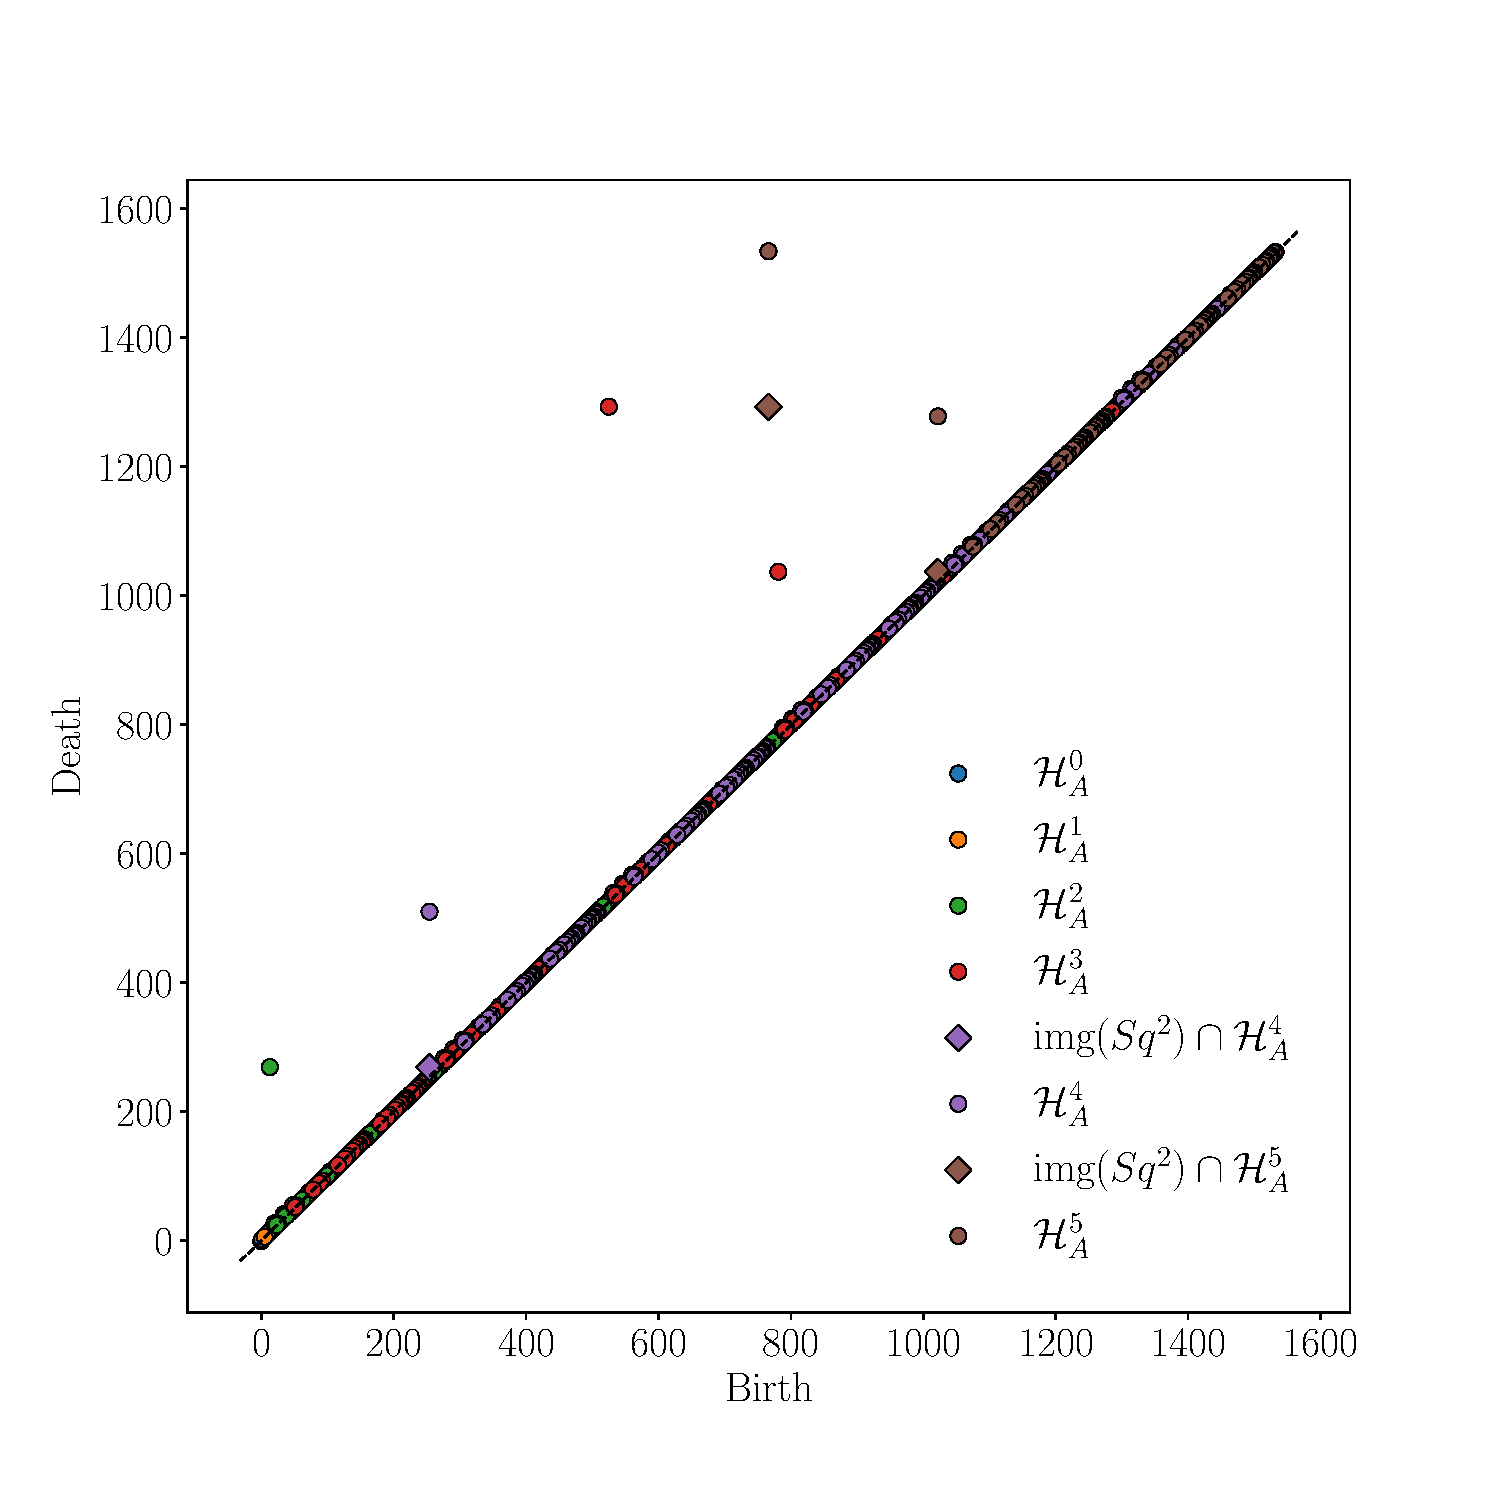
\includegraphics[width=\textwidth]{aux/cp2.pdf}
			\caption{$\mathrm C\,\Sigma\,\mathbb C \mathrm P^2$}
			\label{f:cp2}
		\end{subfigure}
	\end{figure}
\end{frame}

\begin{frame}{Shortcomings of Betti numbers}
	\pause
	Barcodes are based on the \colorit{Betti numbers} of spaces, the $\beta_d$'s.

	\pause\medskip
	But these \colorit{forget} much information.
	\pause For \pcolor{example}, if $K$ is the Klein bottle
	\begin{center}
		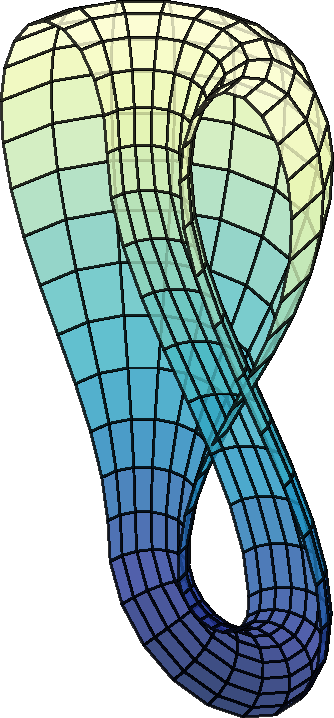
\includegraphics[scale=.3]{aux/KB.pdf}
	\end{center}
	over the field with two elements $\Ftwo$ we have
	\[
	\beta_0(K) = 1, \quad \beta_1(K) = 2, \quad \beta_2(K) = 1, \quad \beta_i(K) = 0.
	\]
	The same as the torus $T$.
\end{frame}

\begin{frame}{Steenrod squares}
	\pause
	For each $k$ there are natural maps
	\[
	\Sq^k \colon H^d(X;\Ftwo) \to H^{d+k}(X,\Ftwo).
	\]

	\pause
	$\Sq^1$ \pcolor{distinguishes} the torus and the Klein bottle
	\begin{figure}
		\newcommand*{\xMin}{0}%
\newcommand*{\xMax}{4}%
\newcommand*{\yMin}{0}%
\newcommand*{\yMax}{4}%
%\only<2>{
%\vskip4pt
%\begin{center}
%	\centering
%	\begin{tikzpicture}[scale=.6]
%		\draw[-{Latex[length=2mm]}] (-.5,\yMin)--(-.5,\yMax);
%		\draw[-{Latex[length=2mm]}] (-.5,\yMin)--(-.5,\yMax-.5);
%		\draw[-{Latex[length=2mm]}] (4.5,\yMin)--(4.5,\yMax);
%		\draw[-{Latex[length=2mm]}] (4.5,\yMin)--(4.5,\yMax-.5);
%
%		\draw[-{Latex[length=2mm]}] (\xMin, -.5)--(\xMax, -.5);
%		\draw[-{Latex[length=2mm]}] (\xMin, 4.5)--(\xMax, 4.5);
%
%		\draw (0,0)--(0,4)--(4,4)--(4,0)--(0,0);
%
%		\node at (2,5.3){Torus};
%		\node at (2,-1.3){\phantom{$\rank \Sq^1 = 0$}};
%	\end{tikzpicture}
%	\hspace*{2cm}
%	\begin{tikzpicture}[scale=.6]
%		\draw[-{Latex[length=2mm]}] (-.5,\yMin)--(-.5,\yMax);
%		\draw[-{Latex[length=2mm]}] (-.5,\yMin)--(-.5,\yMax-.5);
%		\draw[-{Latex[length=2mm]}] (4.5,\yMax)--(4.5,\yMin);
%		\draw[-{Latex[length=2mm]}] (4.5,\yMax)--(4.5,\yMin+.5);
%
%		\draw[-{Latex[length=2mm]}] (\xMin, -.5)--(\xMax, -.5);
%		\draw[-{Latex[length=2mm]}] (\xMin, 4.5)--(\xMax, 4.5);
%
%		\draw (0,0)--(0,4)--(4,4)--(4,0)--(0,0);
%
%		\node at (2,5.3){Klein Bottle };
%		\node at (2,-1.3){\phantom{$\rank \Sq^1 = 1$}};
%	\end{tikzpicture}
%	%	\caption{Klein Bottle. $\rank \Sq^1 = 0$}
%\end{center}}
\pause
\begin{center}
	\centering
	\begin{tikzpicture}[scale=.6]
		\draw[-{Latex[length=2mm]}] (-.5,\yMin)--(-.5,\yMax);
		\draw[-{Latex[length=2mm]}] (-.5,\yMin)--(-.5,\yMax-.5);
		\draw[-{Latex[length=2mm]}] (4.5,\yMin)--(4.5,\yMax);
		\draw[-{Latex[length=2mm]}] (4.5,\yMin)--(4.5,\yMax-.5);

		\draw[-{Latex[length=2mm]}] (\xMin, -.5)--(\xMax, -.5);
		\draw[-{Latex[length=2mm]}] (\xMin, 4.5)--(\xMax, 4.5);

		\draw (0,0)--(0,4)--(4,4)--(4,0)--(0,0);

		\draw[color=blue!50, very thick] (0,2) .. controls (1,2.5) and (3,1.5) .. (4,2);
		\draw[color=red!50, very thick] (0,1) .. controls (1,1.3) and (3,1) .. (4,1);

		\node at (2,5.3){$T$};
		\node at (2,-1.3){$\rank \Sq^1 = 0$};
	\end{tikzpicture}
	\hspace*{2cm}
	\begin{tikzpicture}[scale=.6]
		\draw[-{Latex[length=2mm]}] (-.5,\yMin)--(-.5,\yMax);
		\draw[-{Latex[length=2mm]}] (-.5,\yMin)--(-.5,\yMax-.5);
		\draw[-{Latex[length=2mm]}] (4.5,\yMax)--(4.5,\yMin);
		\draw[-{Latex[length=2mm]}] (4.5,\yMax)--(4.5,\yMin+.5);

		\draw[-{Latex[length=2mm]}] (\xMin, -.5)--(\xMax, -.5);
		\draw[-{Latex[length=2mm]}] (\xMin, 4.5)--(\xMax, 4.5);

		\draw (0,0)--(0,4)--(4,4)--(4,0)--(0,0);

		\draw[color=blue!50, very thick] (0,2) .. controls (1,2.5) and (3,1.5) .. (4,2);
		\draw[color=red!50, very thick] (0,1) .. controls (1,1) and (2,2.5) .. (4,3);

		\node at (2,5.3){$K$};
		\node at (2,-1.3){$\rank \Sq^1 = 1$};
	\end{tikzpicture}
%	\caption{Klein Bottle. $\rank \Sq^1 = 0$}
\end{center} % REMEMBER TO UNCOMMENT INSIDE
	\end{figure}
\end{frame}

\begin{frame}{Computing Steenrod squares}
	\pause

	\colorit{Contribution (Med.)}: A faster way to compute $\Sq^k$ for simplicial complexes.

	\pause\medskip
	\pcolor{Example}: Clocking the computation of \colorit{$\Sq^1$}, the old and new ways.
	\vspace*{10pt}

	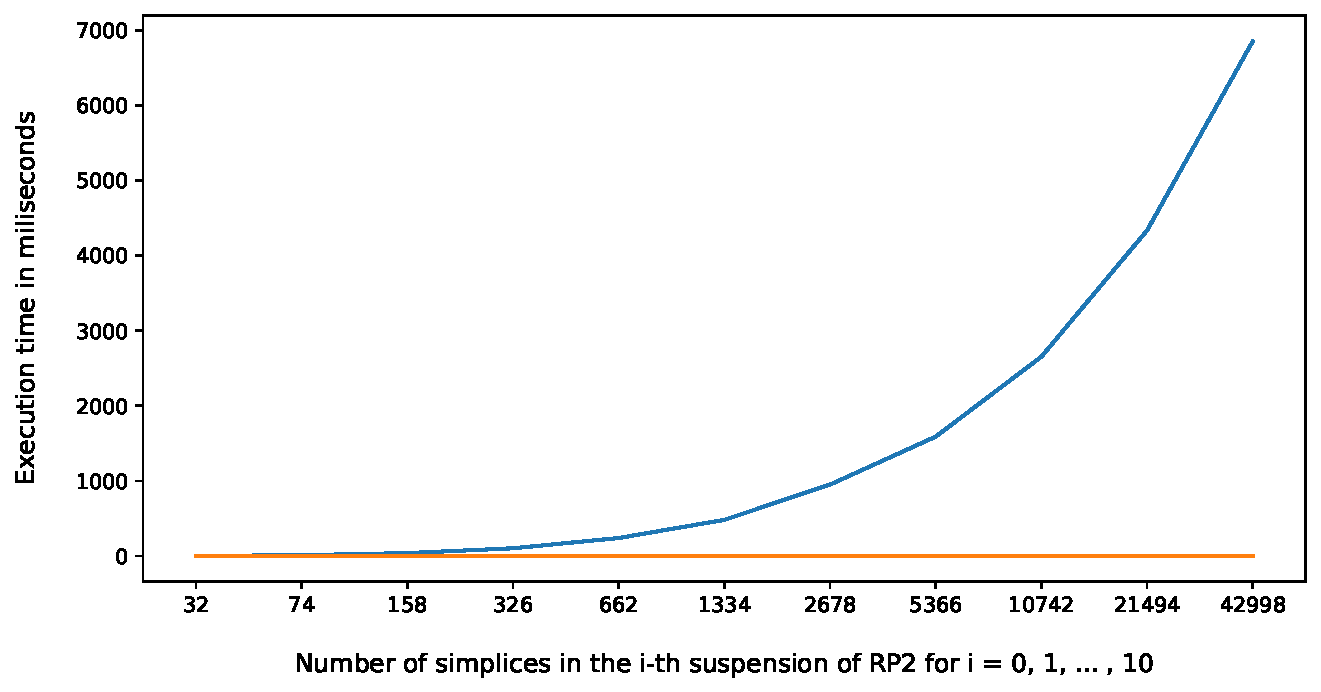
\includegraphics[width=\textwidth]{aux/comp_sus_rp2.pdf}
\end{frame}

\begin{frame}[fragile]{Persistent Steenrod squares}
	\pause
	Given a filtered simplicial complex
	\begin{equation}\label{eq:filtration}
		X_0 \subset X_1 \subset \cdots \subset X_n,
	\end{equation}

	\pause\smallskip
	For each $k$ and $d$, $\Sq^k$ induces a family of compatible linear maps
	\[
	\begin{tikzcd}[column sep = 15]
		H^d(X_n; \Ftwo) \arrow[d, "\Sq^k"] \arrow[r] & \cdots \arrow[r] & H^d(X_{n-1}; \Ftwo) \arrow[d, "\Sq^k"] \arrow[r] & H^d(X_0; \Ftwo) \arrow[d, "\Sq^k"]  \\
		H^{d+k}(X_n; \Ftwo) \arrow[r] & \cdots \arrow[r] & H^{d+k}(X_{n-1}; \Ftwo) \arrow[r] & H^{d+k}(X_0; \Ftwo).
	\end{tikzcd}
	\]

	\pause
	\colorit{Definition (Lupo--Med.--Tauzin)} \\
	The \colorit{$\Sq^k$ barcode} of (1) is defined as the barcode of $\mathrm{img}\ \Sq^k$.

	\pause\bigskip
	\colorit{Theorem (Ling Zhou--Med.--M\'emoli)} \\
	These barcodes are stable.

	\pause\bigskip
	\colorit{Computable}?
\end{frame}

\begin{frame}{\texttt{Steenroder}}
	\pause

	A ready-to-use \colorit{package} for computing Steenrod barcodes.

	\begin{center}
		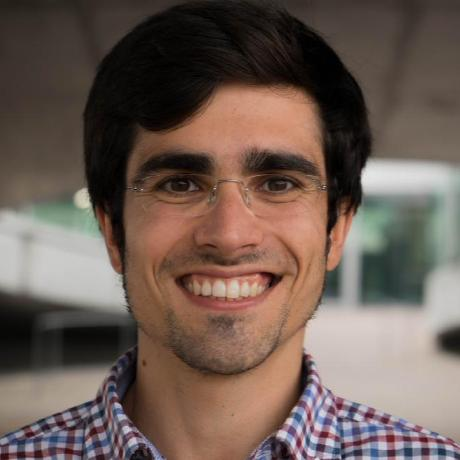
\includegraphics[scale=.1]{aux/umberto}
		\qquad
		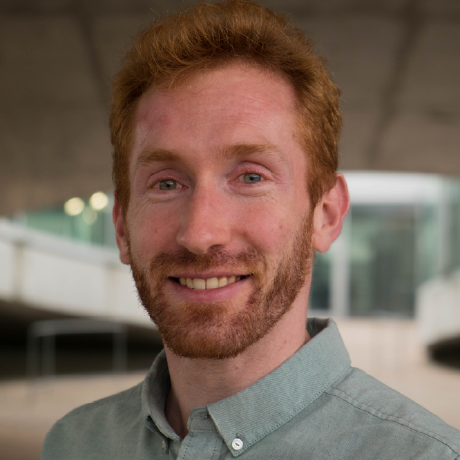
\includegraphics[scale=.1]{aux/guillaume}
	\end{center}

	Developed with \textit{U. Lupo} and \textit{G.~Tauzin} from \raisebox{-1pt}{
\includegraphics[scale=0.1]{aux/giotto.png}}.

	\begin{center}
		\hyperlink{https.github.com/Steenroder/steenroder.com}{github.com/Steenroder/steenroder}
	\end{center}

	\pause\bigskip
	\colorit{Question:} Are these finer invariants out there in the real world?
\end{frame}

%\begin{frame}{Example: $\Sq^2$}
%	\pause
%	Filtrations of the cone on $\Sigma(S^2 \vee S^4)$ and $\Sigma \bC \rP^2$.
%
%	\pause
%	\begin{figure}
%		\centering
%		\begin{subfigure}[b]{0.49\textwidth}
%			\centering
%			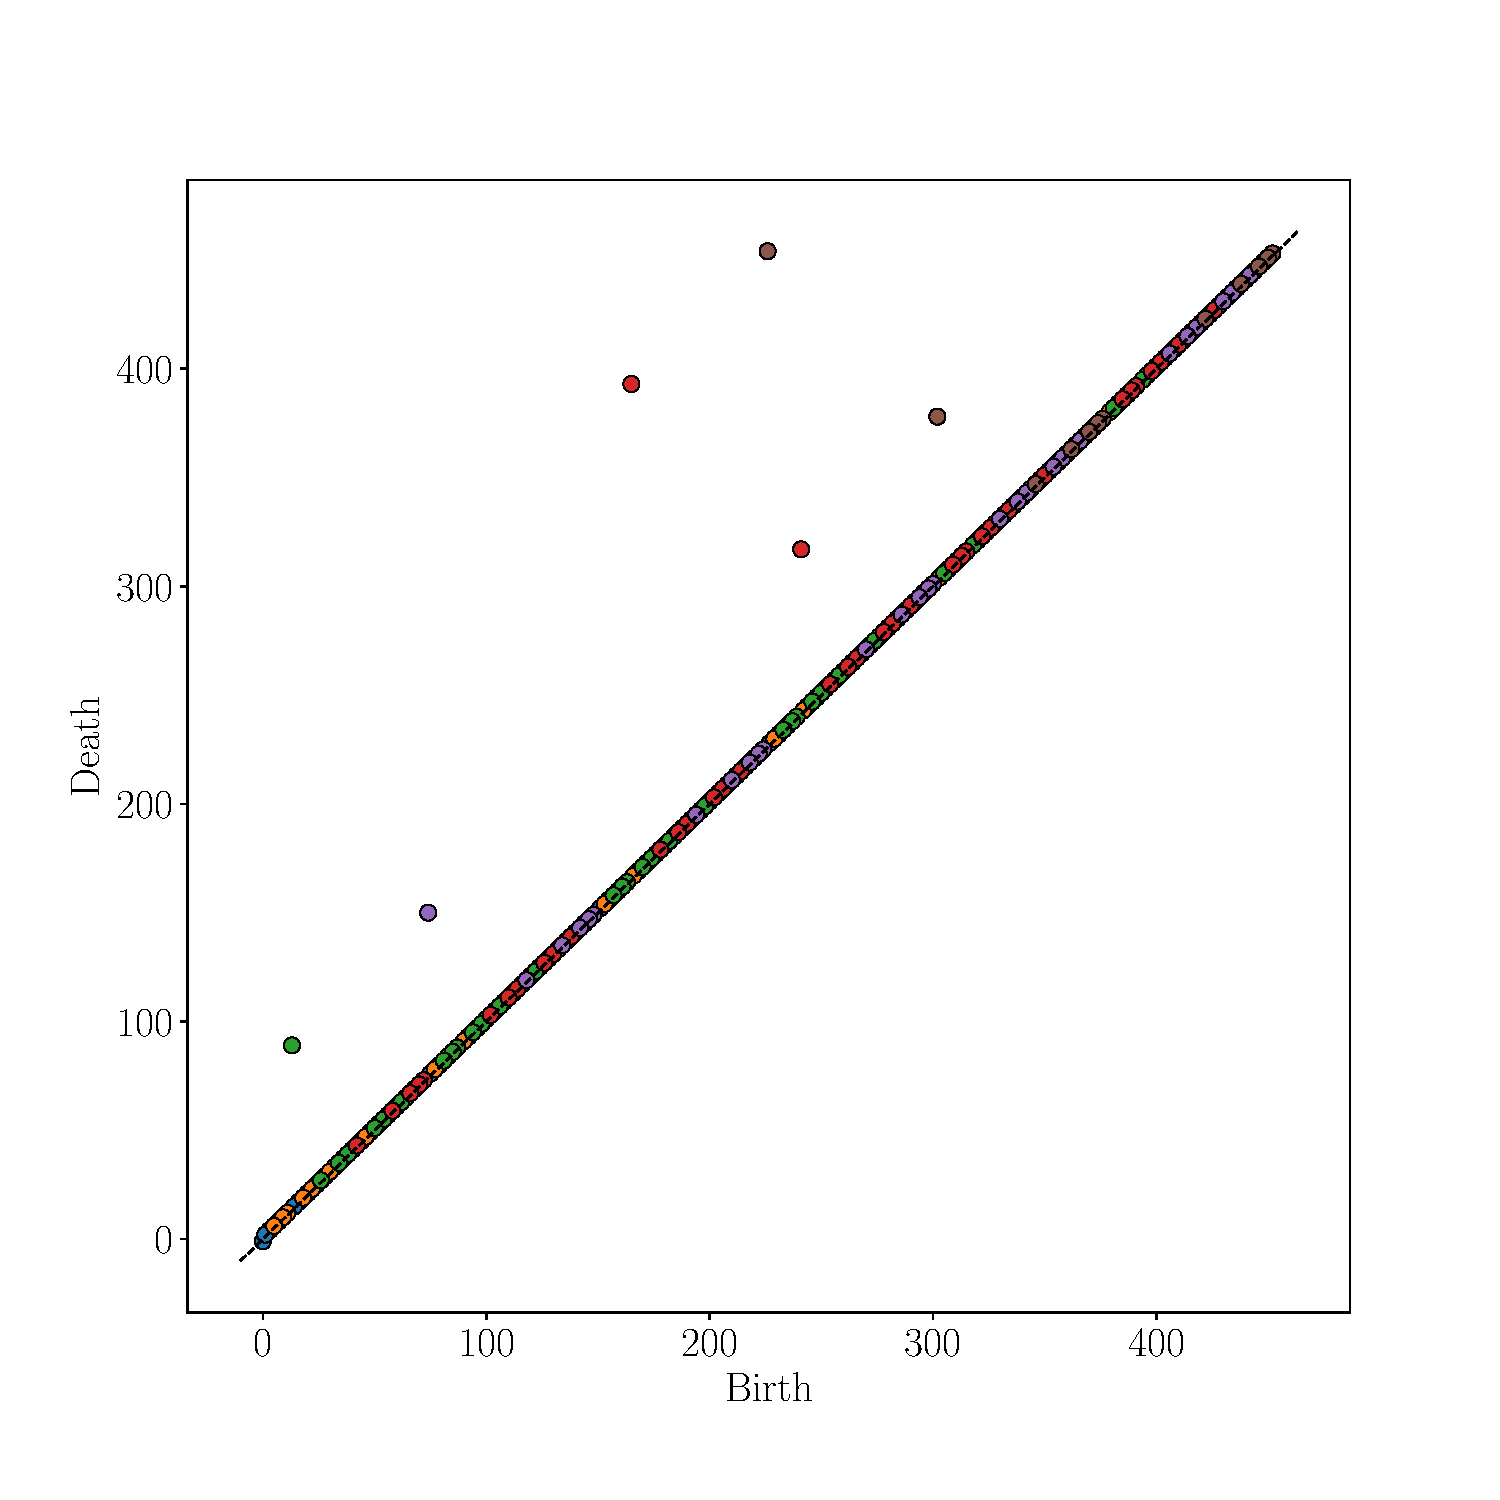
\includegraphics[width=\textwidth]{aux/s2_s4.pdf}
%			\caption{$\mathrm C\,\Sigma(S^2 \vee S^4)$}
%			\label{f:s2_s4}
%		\end{subfigure}
%		\begin{subfigure}[b]{0.49\textwidth}
%			\centering
%			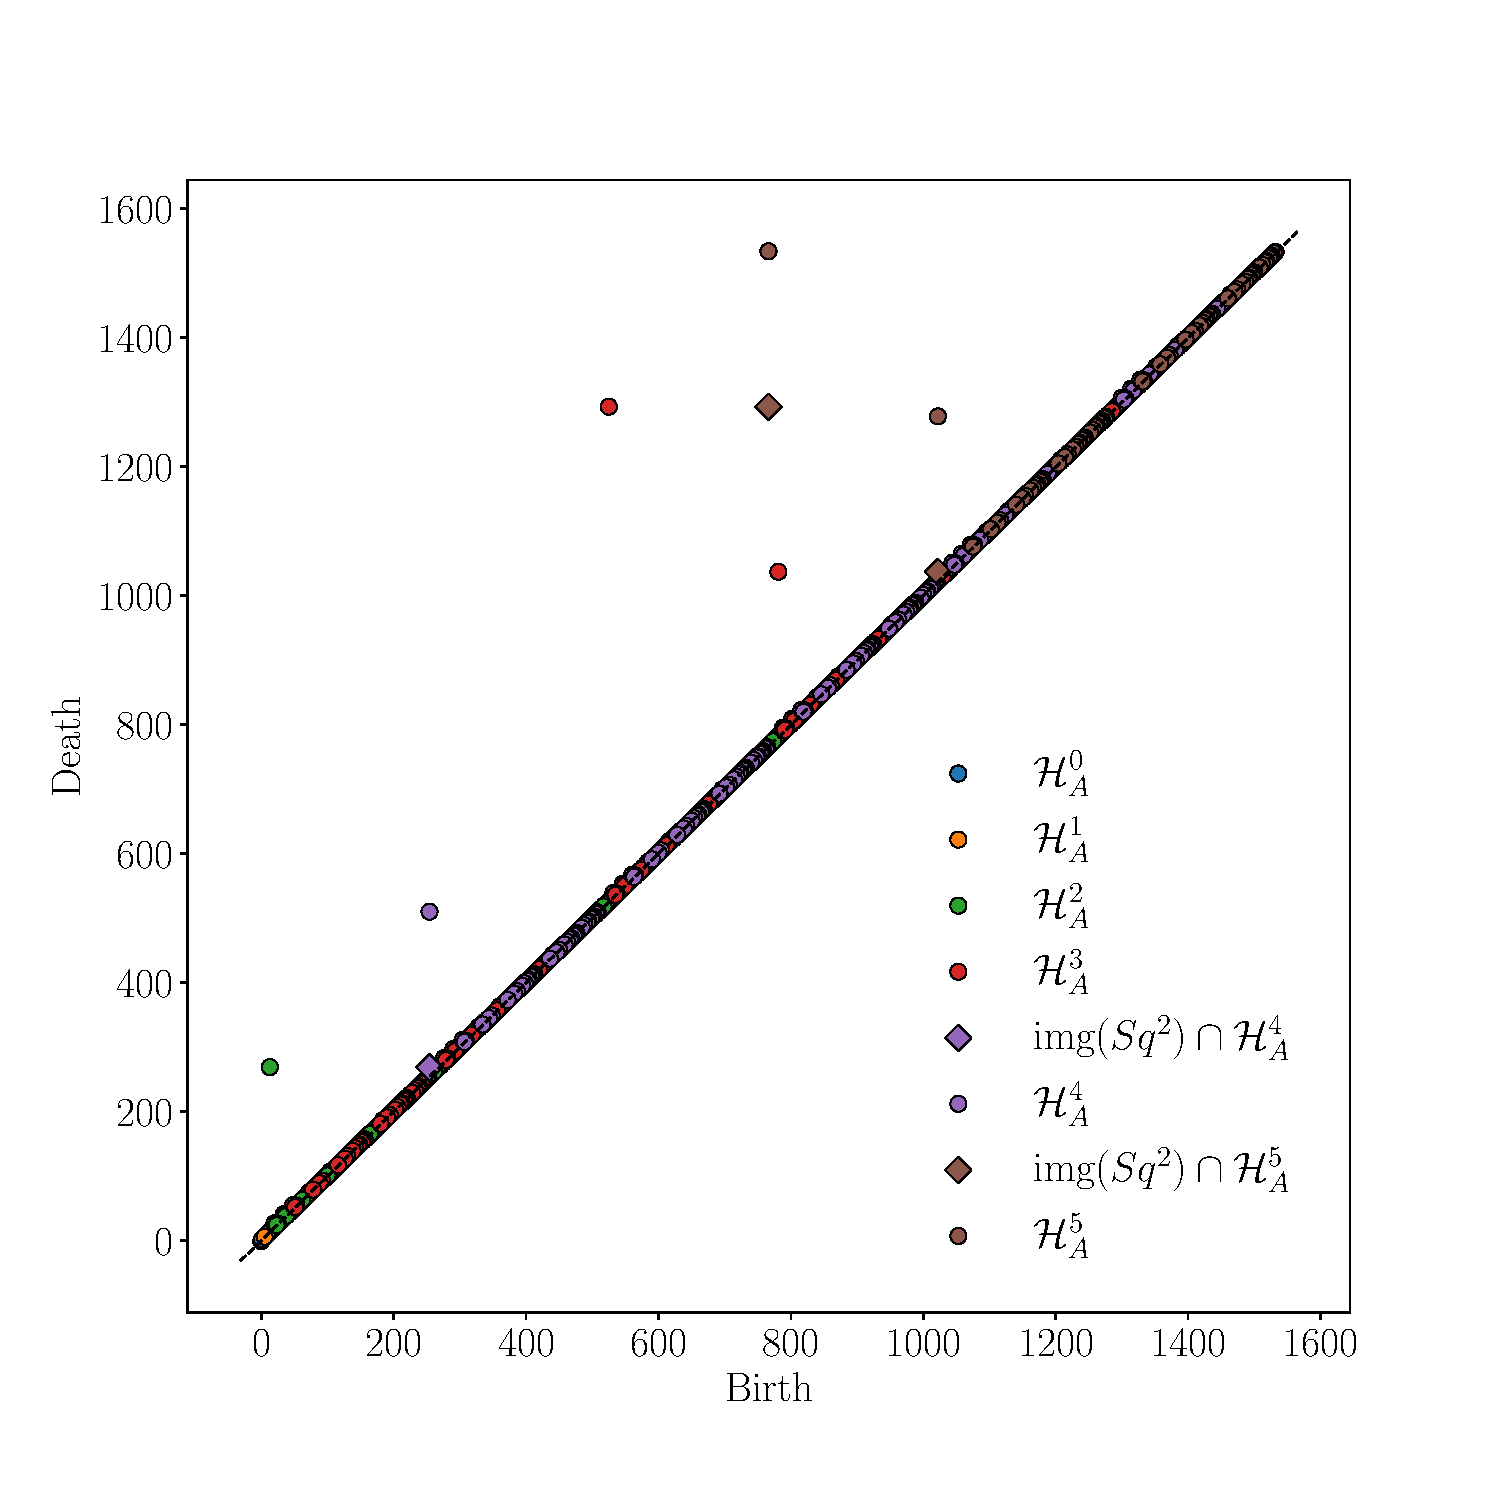
\includegraphics[width=\textwidth]{aux/cp2.pdf}
%			\caption{$\mathrm C\,\Sigma\,\bC\rP^2$}
%			\label{f:cp2}
%		\end{subfigure}
%	\end{figure}
%\end{frame}

\begin{frame}{Space of conformations of $\mathrm{C_8H_{16}}$}
	\pause
	Points in $\R^{24}$ (positions of $8$ carbons in $\R^3$)

	\pause\medskip
	$H^1$ (green) and $H^2$ (blue) barcodes of (part of) this point cloud
	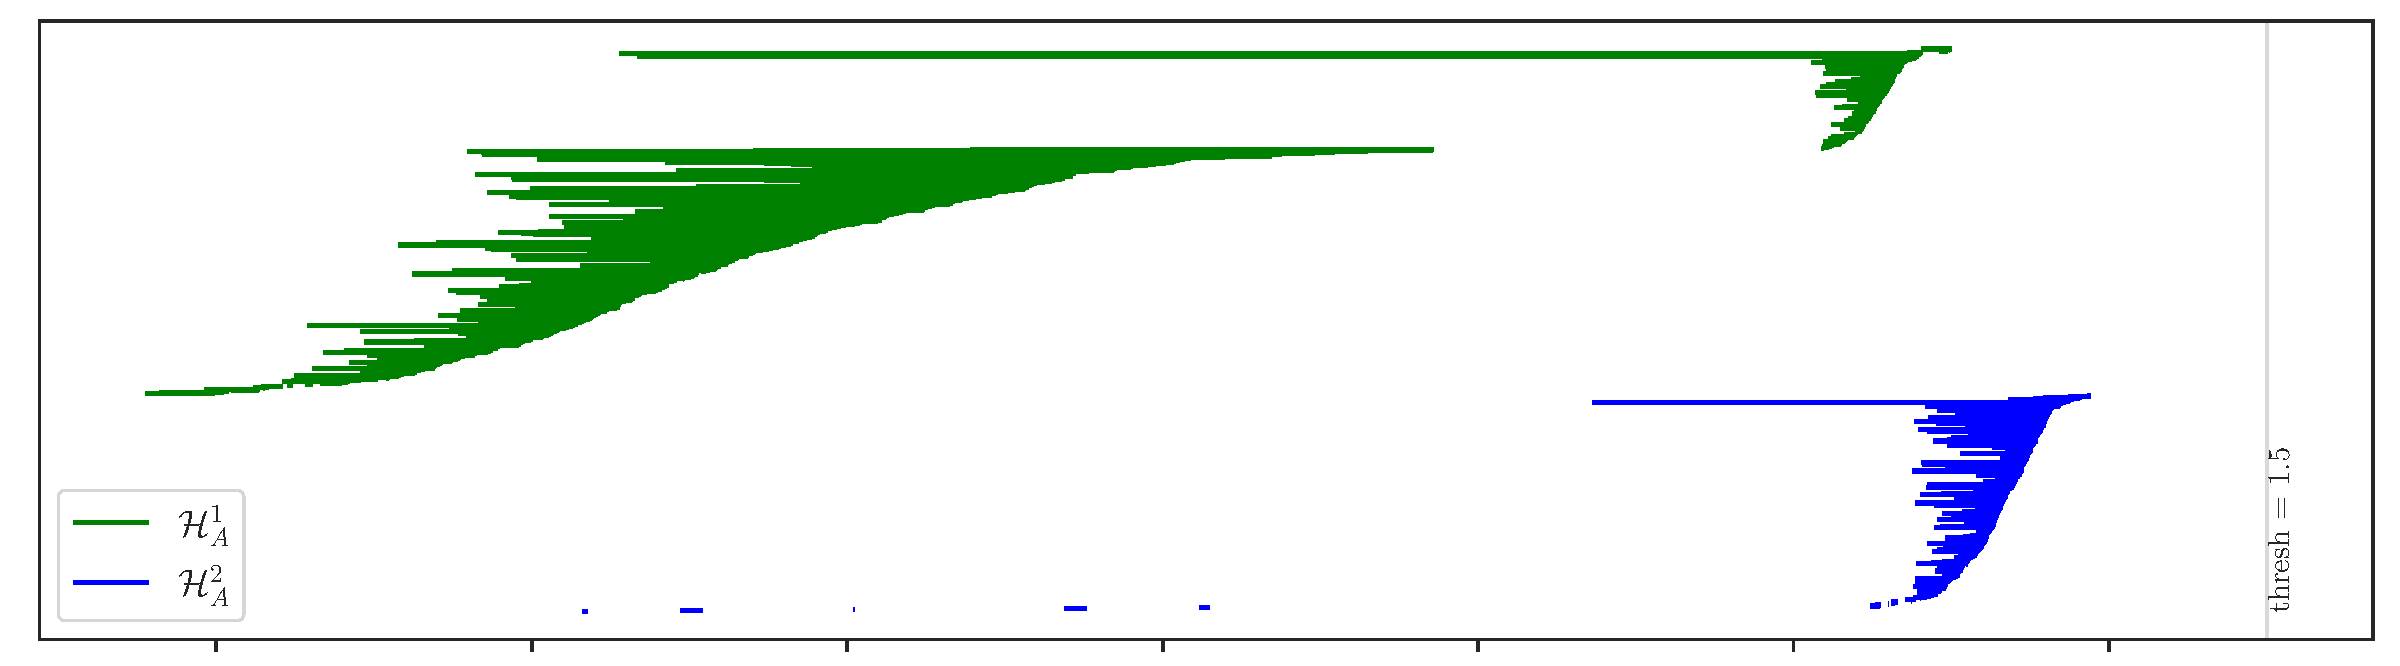
\includegraphics[width=\textwidth]{aux/molecule_top.pdf}

	\pause
	$\Sq^1$ barcode
	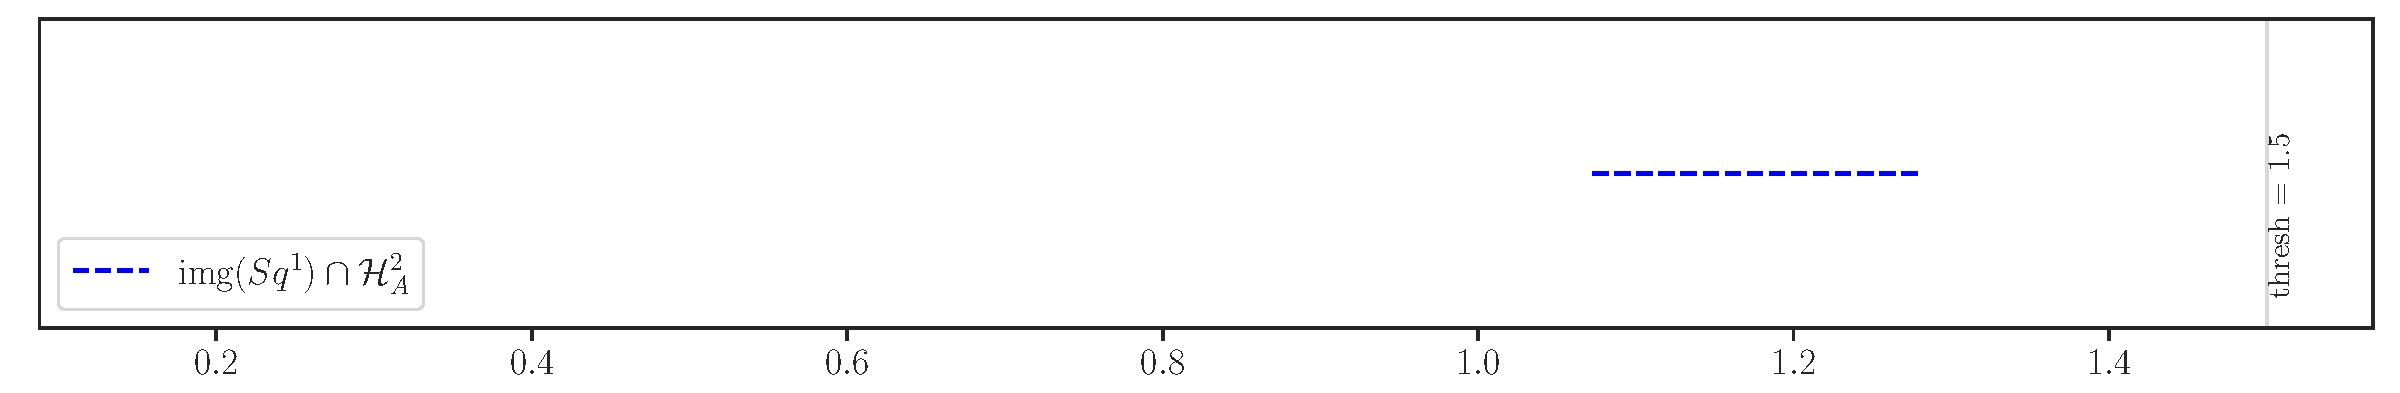
\includegraphics[width=\textwidth]{aux/molecule_bot.pdf}
	Consistent with a \colorit{Klein bottle}.
\end{frame}

\begin{frame}{Summary}
	Persistent homology and their Steenrod generalization are principled tools for feature extraction.

	\pause\medskip
	\begin{itemize}
		\itemsep15pt % Adjusts the space between items
		\item They capture the primitive \pcolor{shape} of data.

		\item They are relevant at \pcolor{multiple scales}.

		\item Their output, barcodes, form a \pcolor{metric space}.

		\item They are \pcolor{robust} to noise.

		\item They are \pcolor{computable} in practice: \texttt{giotto-tda} - \texttt{steenroder}.

		\item They are useful in the study \pcolor{real-world data}.
	\end{itemize}
\end{frame}